\documentclass{beamer}

\usepackage[T1]{fontenc}
\usepackage[utf8]{inputenc}
\usepackage{amsmath,amssymb,amsfonts}
\usepackage{physics}
\usepackage{bm}
\usepackage{mathtools}
\usepackage{tikz}
\usetikzlibrary{quantikz,arrows.meta,positioning}

\title{The Quantum Approximate Optimization Algorithm (QAOA)}
\subtitle{From Foundations to Gradient Methods}
\author{Morten Hjorth-Jensen}
\date{Spring 2026}

\begin{document}

\frame{\titlepage}

%------------------------------------------------
\begin{frame}{Outline}
\begin{enumerate}
\item Combinatorial optimization and the QUBO/Ising mapping
\item Variational quantum algorithms and VQE
\item Definition and structure of QAOA
\item Adiabatic origins and Trotterization
\item MaxCut: explicit construction and gate decomposition
\item Analytic solution at $p=1$
\item Performance, landscape, and limitations
\item Statistical mechanics and control-theoretic connections
\item Gradient methods for QAOA optimization
\item Summary and outlook
\end{enumerate}
\end{frame}


%================================================
\section{Combinatorial Optimization}
%================================================

\begin{frame}{The Optimization Problem}
Many problems in physics and computer science reduce to optimizing a
cost function over discrete variables:
\[
\min_{z \in \{0,1\}^n} C(z)
\]

Concrete examples:
\begin{itemize}
\item Ground-state energy minimization in spin models
\item MaxCut, satisfiability (SAT), traveling salesman
\item Scheduling, portfolio optimization
\end{itemize}

These are in general \textbf{NP-hard}: exact solutions scale exponentially with
system size $n$. Approximate algorithms aim for a ratio
\[
\alpha = \frac{C(x^*)}{C_{\max}} \lesssim 1.
\]
\end{frame}

%------------------------------------------------

\begin{frame}{QUBO Formulation}
A natural discrete framework is Quadratic Unconstrained Binary
Optimization (QUBO):
\[
C(x) = x^T Q\, x = \sum_{i,j} Q_{ij}\, x_i x_j, \qquad
x^* = \arg\min_{x \in \{0,1\}^n} C(x).
\]

Mapping to Ising variables $z_i = 2x_i - 1 \in \{-1,+1\}$ turns the
cost function into a \emph{Hamiltonian}:
\[
\hat{H}_C = \sum_{i<j} J_{ij}\, Z_i Z_j + \sum_i h_i\, Z_i.
\]

This QUBO $\leftrightarrow$ Ising equivalence enables quantum
optimization: the ground state of $\hat{H}_C$ encodes the optimal
solution. It is also the basis for both quantum annealing and QAOA.
\end{frame}

%------------------------------------------------

\begin{frame}{MaxCut: A Benchmark Problem}
Given a weighted graph $G=(V,E)$, partition the vertices into two
sets to maximize the total weight of cut edges:
\[
C(x) = \sum_{(i,j)\in E} w_{ij}\, x_i(1-x_j).
\]

MaxCut is NP-hard and a standard benchmark for quantum optimization.

\medskip

\textbf{Quantum Hamiltonian.} Using $x_i = (1-Z_i)/2$:
\[
\hat{H}_C = \frac{1}{2}\sum_{(i,j)\in E} w_{ij}(I - Z_i Z_j).
\]

The ground state of $\hat{H}_C$ encodes the optimal cut.

\medskip

\textbf{Classical baseline.} The Goemans--Williamson semidefinite
programming algorithm achieves approximation ratio $\alpha \approx
0.878$.
\end{frame}

%------------------------------------------------

\begin{frame}{Classical Optimization Methods}
Solving the optimization problem classically:
\begin{itemize}
\item \textbf{Exact methods:} branch-and-bound, integer programming
  --- exponential worst-case cost.
\item \textbf{Approximation algorithms:} semidefinite programming
  (Goemans--Williamson, $\alpha\approx 0.878$ for MaxCut).
\item \textbf{Heuristics:} simulated annealing, genetic algorithms,
  greedy methods --- no guarantee on quality.
\end{itemize}

\medskip

Quantum computing offers a potentially different route: use quantum
interference and entanglement to explore the configuration space
coherently. QAOA is the leading near-term proposal.
\end{frame}


%================================================
\section{Variational Quantum Algorithms}
%================================================

\begin{frame}{Variational Quantum Algorithms (VQAs)}
The variational principle underpins a broad class of
\textbf{hybrid quantum-classical} algorithms:

\begin{enumerate}
\item Prepare a parameterized quantum state
  $|\psi(\boldsymbol{\theta})\rangle = U(\boldsymbol{\theta})|0\rangle$.
\item Measure the expectation value
  $E(\boldsymbol{\theta}) = \langle\psi(\boldsymbol{\theta})|\hat{H}|\psi(\boldsymbol{\theta})\rangle$
  on the quantum device.
\item Update $\boldsymbol{\theta}$ with a classical optimizer.
\item Repeat until convergence.
\end{enumerate}

The quantum device handles the state preparation and measurement; the
classical computer handles the optimization.
\end{frame}

%------------------------------------------------

\begin{frame}{Variational Quantum Eigensolver (VQE)}
VQE is the prototypical VQA for finding ground-state energies:
\[
E_0 \approx \min_{\boldsymbol{\theta}}
\langle\psi(\boldsymbol{\theta})|\hat{H}|\psi(\boldsymbol{\theta})\rangle.
\]

Key ingredients:
\begin{itemize}
\item A \textbf{flexible ansatz} $U(\boldsymbol{\theta})$ --- the
  circuit structure is chosen by the user.
\item Measurement of expectation values via Pauli decomposition.
\item A classical optimizer (gradient-based or gradient-free).
\end{itemize}

\medskip

QAOA is a \emph{special case} of VQE where the ansatz is
\textbf{problem-inspired} and fixed by the structure of the
cost Hamiltonian, rather than chosen freely.
\end{frame}


%================================================
\section{QAOA: Definition and Structure}
%================================================

\begin{frame}{Motivation for QAOA}
We want to solve
\[
\min_{z\in\{0,1\}^n} C(z)
\]
using a quantum circuit that is both \emph{shallow} (NISQ-compatible)
and \emph{structured} (informed by the problem).

\medskip

Two key observations:
\begin{itemize}
\item The cost function can be encoded as a diagonal Hamiltonian
  $H_C = \sum_z C(z)|z\rangle\langle z|$.
\item Alternating evolution under $H_C$ and a mixing Hamiltonian $H_M$
  can explore the solution space coherently.
\end{itemize}

QAOA formalizes this into a variational circuit with $2p$ free
parameters.
\end{frame}

%------------------------------------------------

\begin{frame}{QAOA: Formal Definition}
QAOA constructs the parameterized state
\[
|\psi_p(\boldsymbol{\gamma},\boldsymbol{\beta})\rangle
=
\prod_{k=1}^{p}
e^{-i\beta_k H_M}\,
e^{-i\gamma_k H_C}
\,|\!+\rangle^{\otimes n},
\]
where:
\begin{itemize}
\item $H_C$: cost Hamiltonian encoding the objective function,
\item $H_M = \sum_{i=1}^n X_i$: mixing Hamiltonian,
\item $p$: circuit depth (number of layers),
\item $\boldsymbol{\gamma} = (\gamma_1,\dots,\gamma_p)$,
  $\boldsymbol{\beta} = (\beta_1,\dots,\beta_p)$: variational parameters.
\end{itemize}

The objective is to maximize the expectation value:
\[
F_p(\boldsymbol{\gamma},\boldsymbol{\beta})
= \langle\psi_p|\,H_C\,|\psi_p\rangle,
\qquad
(\boldsymbol{\gamma}^*,\boldsymbol{\beta}^*) = \arg\max\, F_p.
\]
\end{frame}

%------------------------------------------------

\begin{frame}{Initial State and Hamiltonians}
\textbf{Initial state.}
The algorithm starts from the equal superposition of all bitstrings:
\[
|+\rangle^{\otimes n}
= \frac{1}{2^{n/2}}\sum_{z\in\{0,1\}^n}|z\rangle,
\]
which is the ground state of $-H_M$ and represents complete ignorance
about the solution.

\medskip

\textbf{Cost Hamiltonian.}
The cost function is encoded as a diagonal operator:
\[
H_C = \sum_z C(z)\,|z\rangle\langle z|.
\]
In Ising form: $H_C = \sum_{i<j}J_{ij}Z_iZ_j + \sum_i h_i Z_i$.

\medskip

\textbf{Mixer Hamiltonian.}
The standard choice $H_M = \sum_i X_i$ generates transitions between
computational basis states and ensures exploration of the search space.
\end{frame}

%------------------------------------------------

\begin{frame}{QAOA Circuit Structure}
Each of the $p$ layers consists of two unitaries:
\[
U_C(\gamma_k) = e^{-i\gamma_k H_C}, \qquad
U_M(\beta_k) = e^{-i\beta_k H_M}.
\]

The full circuit is:

\medskip
\centering
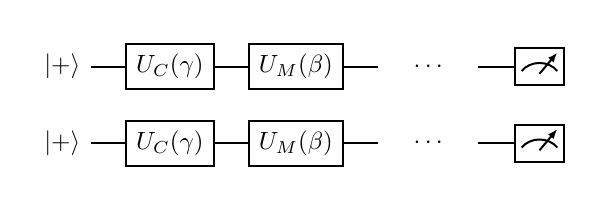
\begin{tikzpicture}
\node[scale=0.9]{
\begin{quantikz}[row sep=0.4cm, column sep=0.5cm]
\lstick{$|+\rangle$} & \gate{U_C(\gamma)} & \gate{U_M(\beta)} & \qw & \cdots & & \meter{} \\
\lstick{$|+\rangle$} & \gate{U_C(\gamma)} & \gate{U_M(\beta)} & \qw & \cdots & & \meter{}
\end{quantikz}
};
\end{tikzpicture}

\medskip
\raggedright
Repeated $p$ times. The approximation ratio is
\[
\alpha = \frac{F_p(\boldsymbol{\gamma}^*,\boldsymbol{\beta}^*)}{C_{\max}}.
\]
\end{frame}

%------------------------------------------------

\begin{frame}{Ansatz Variants}
The standard QAOA ansatz can be extended:
\begin{itemize}
\item \textbf{Multi-angle QAOA:} independent parameters for each gate,
  increasing expressivity.
\item \textbf{Adaptive QAOA:} problem-specific ansatz construction,
  building the circuit layer by layer.
\item \textbf{Counterdiabatic QAOA:} adds correction terms inspired by
  counterdiabatic driving to speed up convergence.
\end{itemize}

All variants share the same hybrid quantum-classical optimization loop
and the same underlying physical motivation.
\end{frame}


%================================================
\section{Adiabatic Origins and Trotterization}
%================================================

\begin{frame}{Quantum Adiabatic Algorithm (QAA)}
The Quantum Adiabatic Algorithm solves optimization problems by
\emph{slow} continuous evolution under a time-dependent Hamiltonian:
\[
\hat{H}(s) = (1-s)\,H_M + s\,H_C, \qquad s = t/T \in [0,1].
\]

\textbf{Adiabatic theorem:} if the evolution is slow enough (relative
to the inverse spectral gap), the system remains in the ground state
throughout, so:
\[
|\psi(T)\rangle
= \mathcal{T}\exp\!\left(-i\!\int_0^T\!\hat{H}(t)\,dt\right)|s\rangle
\;\xrightarrow{T\to\infty}\;
|\text{ground state of }H_C\rangle.
\]

The bottleneck is the required time $T \sim 1/\Delta^2$, where $\Delta$
is the minimum spectral gap.
\end{frame}

%------------------------------------------------

\begin{frame}{Trotterizing the Adiabatic Evolution}
Discretize the time interval into $p$ steps of size $\Delta t = T/p$:
\[
U(T) \approx \prod_{k=1}^p
e^{-i\Delta t\,\hat{H}(s_k)}.
\]

Apply the Trotter--Suzuki decomposition,
$e^{-i(A+B)\Delta t} \approx e^{-iA\,\Delta t}\,e^{-iB\,\Delta t}$,
to each step:
\[
U(T) \approx \prod_{k=1}^p
e^{-i\gamma_k H_C}\,e^{-i\beta_k H_M},
\]
where $\gamma_k \sim s_k\,\Delta t$ and $\beta_k \sim
(1-s_k)\,\Delta t$.

\[
\boxed{\text{QAOA is a Trotterized (discretized) adiabatic evolution.}}
\]
\end{frame}

%------------------------------------------------

\begin{frame}{From Fixed Schedule to Free Parameters}
The adiabatic algorithm uses a \textbf{fixed} schedule $s(t)$.
QAOA replaces it with \textbf{free variational parameters}:
\[
(\gamma_k, \beta_k) \text{ are optimized classically.}
\]

Advantages of the variational approach:
\begin{itemize}
\item No need for a slow, hardware-expensive evolution.
\item Adapts to hardware noise and connectivity.
\item Can outperform the naive adiabatic schedule for finite $p$.
\end{itemize}

\textbf{Limit $p\to\infty$:}
\[
\lim_{p\to\infty}|\psi_p\rangle \to |\psi_{\text{ground}}\rangle.
\]
At finite $p$ we get a shallow, NISQ-compatible circuit.
\end{frame}

%------------------------------------------------

\begin{frame}{Connection to Physics}
QAOA is equivalent to a \textbf{discrete quantum quench sequence}:
alternately freeze the system under $H_C$ for time $\gamma_k$, then
drive it with the mixer $H_M$ for time $\beta_k$.

\medskip

This connects QAOA to:
\begin{itemize}
\item \textbf{Digital quantum simulation} --- Trotterized time evolution.
\item \textbf{Quantum optimal control} --- find the pulse sequence
  $(\gamma_k,\beta_k)$ that maximizes $\langle H_C\rangle$.
\item \textbf{Many-body dynamics} --- the circuit explores entangled
  spin configurations layer by layer.
\end{itemize}
\end{frame}


%================================================
\section{MaxCut: Explicit Construction}
%================================================

\begin{frame}{MaxCut Cost Hamiltonian (Revisited)}
For MaxCut on graph $G=(V,E)$, the classical cost and quantum
Hamiltonian are:
\[
C(z) = \sum_{(i,j)\in E} \frac{1-z_iz_j}{2},
\qquad
H_C = \sum_{(i,j)\in E} \frac{1-Z_iZ_j}{2}.
\]

This is equivalent to an Ising model:
\[
H = -\sum_{(i,j)\in E} J_{ij}\,Z_iZ_j,
\]
so QAOA on MaxCut is exactly a quantum exploration of spin
configurations on the graph. The ground state encodes the maximum cut.
\end{frame}

%------------------------------------------------

\begin{frame}{Gate Decomposition: Cost Unitary}
For one edge $(i,j)$, the cost unitary is
$e^{-i\gamma(1-Z_iZ_j)/2}$.
The non-trivial part is
\[
e^{-i\gamma Z_iZ_j},
\]
implemented by the standard CNOT--$R_Z$--CNOT circuit:

\medskip
\centering
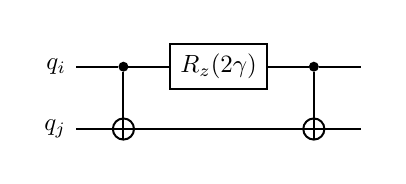
\begin{tikzpicture}
\node[scale=0.9]{
\begin{quantikz}[row sep=0.4cm, column sep=0.5cm]
\lstick{$q_i$} & \ctrl{1} & \gate{R_z(2\gamma)} & \ctrl{1} & \qw \\
\lstick{$q_j$} & \targ{}  & \qw                  & \targ{}  & \qw
\end{quantikz}
};
\end{tikzpicture}

\raggedright
\medskip
One such two-qubit block is applied for every edge in the graph.
\end{frame}

%------------------------------------------------

\begin{frame}{Gate Decomposition: Mixer Unitary}
The mixer $e^{-i\beta H_M} = \prod_i e^{-i\beta X_i}$ is a product of
single-qubit $x$-rotations:
\[
e^{-i\beta X_i} = R_x(2\beta).
\]

\medskip
\centering
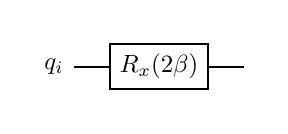
\begin{tikzpicture}
\node[scale=0.9]{
\begin{quantikz}[row sep=0.4cm, column sep=0.5cm]
\lstick{$q_i$} & \gate{R_x(2\beta)} & \qw
\end{quantikz}
};
\end{tikzpicture}

\raggedright
\medskip
Applied independently to every qubit. Together with the cost unitary,
these two building blocks make up a single QAOA layer.
\end{frame}

%------------------------------------------------

\begin{frame}{Classical Optimization Loop}
Once the circuit is built, QAOA runs as a hybrid loop:

\begin{enumerate}
\item \textbf{Initialize} parameters $(\boldsymbol{\gamma},\boldsymbol{\beta})$.
\item \textbf{Run} the quantum circuit and measure
  $\langle H_C\rangle$.
\item \textbf{Update} parameters using a classical optimizer
  (gradient-based or gradient-free).
\item \textbf{Repeat} until convergence.
\end{enumerate}

The quantum device is queried repeatedly; the classical computer
drives the parameter update. The quality of the solution depends
critically on the optimizer choice and initialization.
\end{frame}


%================================================
\section{Analytic Solution at $p=1$}
%================================================

\begin{frame}{Setup: QAOA at $p=1$}
Consider two qubits connected by a single edge, so
\[
H_C = \frac{1-Z_1Z_2}{2}.
\]

The $p=1$ QAOA state is
\[
|\psi(\gamma,\beta)\rangle
= e^{-i\beta H_M}\,e^{-i\gamma H_C}\,|+\rangle^{\otimes 2}.
\]

Apply $U_C(\gamma)$ first: since $Z_1Z_2$ has eigenvalues $\pm 1$,
\[
U_C = e^{-i\gamma/2}\,e^{i\gamma Z_1Z_2/2}.
\]

Then apply $U_M(\beta) = e^{-i\beta(X_1+X_2)} = R_x(2\beta)^{\otimes 2}$.
\end{frame}

%------------------------------------------------

\begin{frame}{Key Computation: Edge Expectation Value}
Carrying out the algebra (a standard result), one finds for a single
edge:
\[
\langle Z_1Z_2\rangle = \sin(4\beta)\sin(2\gamma).
\]

Therefore the expectation value of the cost Hamiltonian is
\[
F(\gamma,\beta) = \langle H_C\rangle
= \frac{1}{2}\bigl(1 - \sin(4\beta)\sin(2\gamma)\bigr).
\]

For a general graph, by linearity:
\[
F(\gamma,\beta) = \sum_{(i,j)\in E}\frac{w_{ij}}{2}
\bigl(1 - \sin(4\beta)\sin(2\gamma)\bigr),
\]
where contributions from different edges decouple at $p=1$.
\end{frame}

%------------------------------------------------

\begin{frame}{Optimal Parameters and Approximation Ratio}
The expectation value is maximized at
\[
\beta^* = \frac{\pi}{8}, \qquad \gamma^* = \frac{\pi}{4},
\]
giving
\[
\sin(4\beta^*)\sin(2\gamma^*) = 1.
\]

For triangle-free regular graphs this yields an approximation ratio
\[
\alpha \approx 0.6924,
\]
matching known analytic results from Farhi, Goldstone, and Gutmann.

\medskip

The $p=1$ circuit captures only \emph{short-range} correlations
(depth-1 light cone). Higher $p$ builds long-range correlations and
approaches the adiabatic limit.
\end{frame}

%------------------------------------------------

\begin{frame}{Locality and General Graphs}
An important structural fact: at depth $p$, the QAOA circuit has a
light-cone of radius $p$.

\[
\text{At depth }p: \text{ correlations extend only to distance }p.
\]

Consequently:
\begin{itemize}
\item For small $p$, the expectation value of each edge term depends
  only on its local neighborhood of radius $p$ in the graph.
\item This makes analytic computations tractable for small $p$.
\item It also limits performance on problems with long-range
  correlations unless $p$ is large.
\end{itemize}
\end{frame}


%================================================
\section{Performance, Landscape, and Limitations}
%================================================

\begin{frame}{Performance as a Function of Depth}
\begin{itemize}
\item $p=1$: shallow circuit, limited accuracy, analytically tractable.
\item Larger $p$: better approximation ratio, closer to adiabatic limit.
\item $p\to\infty$: exact solution recovered.
\end{itemize}

Trade-off:
\[
\text{accuracy} \;\longleftrightarrow\; \text{circuit depth (hardware cost)}.
\]

\medskip

On NISQ devices, gate errors and decoherence limit the practical depth.
Noise mitigation and hardware-aware ansätze are active research topics.
\end{frame}

%------------------------------------------------

\begin{frame}{Energy Landscape}
The objective function
\[
E(\boldsymbol{\gamma},\boldsymbol{\beta})
= \langle\psi(\boldsymbol{\gamma},\boldsymbol{\beta})|H_C
|\psi(\boldsymbol{\gamma},\boldsymbol{\beta})\rangle
\]
is a smooth, $2\pi$-periodic function of $2p$ parameters.

Properties:
\begin{itemize}
\item \textbf{Small $p$:} relatively smooth landscape, easy to optimize.
\item \textbf{Large $p$:} exponentially many local minima; landscape
  resembles spin-glass free-energy surfaces.
\end{itemize}

Parameter optimization strategies:
\begin{itemize}
\item Good initialization (e.g., from a lower-$p$ solution).
\item Gradient-based methods (parameter-shift rule).
\item Exploiting symmetries of the cost Hamiltonian.
\end{itemize}
\end{frame}

%------------------------------------------------

\begin{frame}{Barren Plateaus}
A central challenge for large parameterized circuits is the
\textbf{barren plateau} phenomenon: gradients vanish exponentially
with system size,
\[
\mathrm{Var}\!\left[\partial_{\theta_k} E(\boldsymbol{\theta})\right]
\sim \mathcal{O}(b^{-n}), \qquad b > 1.
\]

Consequences:
\begin{itemize}
\item Training becomes exponentially slow for deep, expressive circuits.
\item Gradient-based optimizers stall.
\end{itemize}

Why QAOA is more resistant:
\begin{itemize}
\item The ansatz is \textbf{problem-inspired} --- the structure of
  $H_C$ concentrates relevant correlations.
\item \textbf{Locality} of the circuit (depth-$p$ light cone) limits
  the spread of barren-plateau effects.
\end{itemize}
\end{frame}


%================================================
\section{Statistical Mechanics and Control Theory}
%================================================

\begin{frame}{Optimization as Physics}
Minimizing $C(z)$ is equivalent to finding the ground state of
\[
H_C = \sum_z C(z)\,|z\rangle\langle z|,
\]
which is a classical Ising Hamiltonian. This maps:
\begin{itemize}
\item combinatorial optimization $\leftrightarrow$ spin-system ground state,
\item QAOA $\leftrightarrow$ controlled quantum exploration of spin
  configurations.
\end{itemize}

\medskip

Physical picture:
\begin{itemize}
\item $H_C$ encodes the energy landscape.
\item $H_M$ induces quantum tunneling between spin configurations.
\item The QAOA layers drive the system toward low-energy states via
  constructive quantum interference.
\end{itemize}
\end{frame}

%------------------------------------------------

\begin{frame}{Real-Time vs Imaginary-Time Evolution}
Classical statistical mechanics uses the \textbf{Gibbs state}:
\[
\rho_{\rm Gibbs} \propto e^{-\beta H}, \qquad
Z = \mathrm{Tr}(e^{-\beta H}).
\]

QAOA instead uses \textbf{real-time} unitary evolution:
\[
|\psi\rangle = e^{-i\beta H_M}\,e^{-i\gamma H_C}\,|+\rangle.
\]

The correspondence $t \to -i\beta$ links:
\begin{itemize}
\item imaginary time $\to$ Gibbs sampling / simulated annealing,
\item real time $\to$ quantum interference / coherent dynamics.
\end{itemize}

QAOA exploits quantum \emph{interference} rather than thermal
fluctuations, which is the fundamental distinction from simulated
annealing.
\end{frame}

%------------------------------------------------

\begin{frame}{Relation to Annealing Algorithms}
\begin{center}
\begin{tabular}{lll}
\hline
\textbf{Method} & \textbf{Mechanism} & \textbf{Evolution} \\
\hline
Simulated annealing & thermal fluctuations & stochastic \\
Quantum annealing   & tunneling            & continuous unitary \\
QAOA                & coherent interference & discrete unitary \\
\hline
\end{tabular}
\end{center}

\medskip

QAOA uses \emph{controlled} coherent evolution with variational
parameters, making it more flexible than fixed-schedule annealing
while remaining tractable on finite-depth quantum circuits.
\end{frame}

%------------------------------------------------

\begin{frame}{Control-Theoretic Interpretation}
From a quantum control perspective, QAOA implements a
piecewise-constant control protocol:
\[
U(\boldsymbol{\theta})
= \mathcal{T}\exp\!\left(-i\int_0^T
\bigl[u_1(t)\,H_C + u_2(t)\,H_M\bigr]\,dt\right),
\]
where $u_1, u_2$ are the piecewise-constant controls $(\gamma_k,\beta_k)$.

The optimization objective
\[
\max_{\boldsymbol{\gamma},\boldsymbol{\beta}}
\langle\psi(T)|H_C|\psi(T)\rangle
\]
is a \textbf{quantum optimal control problem}.

\medskip

As $p\to\infty$, QAOA converges to a continuous Schrödinger evolution
and the control problem approaches the adiabatic limit.
\end{frame}


%================================================
\section{Gradient Methods for QAOA}
%================================================

\begin{frame}{The Gradient Problem}
Optimization of the $2p$ parameters requires the gradient
\[
\nabla E
=
\left(
\frac{\partial E}{\partial \gamma_1},
\frac{\partial E}{\partial \beta_1},
\dots,
\frac{\partial E}{\partial \gamma_p},
\frac{\partial E}{\partial \beta_p}
\right).
\]

If the cost Hamiltonian has a Pauli decomposition
$H_C = \sum_{\alpha=1}^K h_\alpha P_\alpha$, then
\[
E(\boldsymbol{\theta})
= \sum_{\alpha=1}^K h_\alpha
\langle\psi(\boldsymbol{\theta})|P_\alpha|\psi(\boldsymbol{\theta})\rangle,
\]
and the gradient becomes a sum over Pauli-string derivatives.

\medskip

\textbf{Central question:} How does one evaluate
$\partial_{\theta_k}\langle P_\alpha\rangle$ efficiently on hardware?
\end{frame}

%------------------------------------------------

\begin{frame}{General Derivative Structure}
Let $|\psi_0\rangle = |+\rangle^{\otimes n}$ and $U(\boldsymbol{\theta})$
be the full QAOA unitary. Then
\[
E(\boldsymbol{\theta})
= \langle\psi_0|U^\dagger(\boldsymbol{\theta})\,H_C\,
U(\boldsymbol{\theta})|\psi_0\rangle.
\]

Each parameter $\theta_k$ appears in a gate
$U_k(\theta_k) = e^{-i\theta_k B_k}$ with generator
$B_k \in \{H_C, H_M\}$. Writing $U = U_{\rm after}\,U_k(\theta_k)\,U_{\rm before}$,
all gradient methods reduce to evaluating derivatives of
$\langle U^\dagger B_k U \rangle$.

\medskip

\textbf{Why is this nontrivial?}
\begin{itemize}
\item Hardware cannot apply $H|\psi\rangle$ directly as a gate.
\item Each gradient evaluation costs $\mathcal{O}(p)$ circuit calls.
\item Many-term Hamiltonians ($K \gg p$) can dominate cost.
\end{itemize}
\end{frame}

%------------------------------------------------

\begin{frame}{A Concrete Test Case: XXZ Spin Chain}
The five gradient methods are compared on the XXZ Hamiltonian:
\[
H_{\rm XXZ}
= \sum_{i=1}^{L-1}
\bigl[J_{xx}(\sigma_i^x\sigma_{i+1}^x + \sigma_i^y\sigma_{i+1}^y)
+ J_z\,\sigma_i^z\sigma_{i+1}^z\bigr]
+ \sum_{i=1}^L h_z\,\sigma_i^z,
\]
with $J_{xx}=1.0$, $J_z=1.5$, $h_z=0.2$, and $L=6$, $p=2$, giving
$N = 2p = 4$ variational parameters and approximately $K \approx 14$
Pauli terms.

The coupling ratio $h_{\max}/h_{\min} = 7.5$ makes this a
non-trivial benchmark for methods that exploit Hamiltonian structure.
\end{frame}

%------------------------------------------------

\begin{frame}{Method 1: Exact Gradient}
The exact gradient formula follows directly from differentiating
the unitary evolution:
\[
\frac{\partial E}{\partial \theta_k}
= i\langle\psi|H_C\,U^\dagger B_k U|\psi\rangle
- i\langle\psi|U^\dagger B_k U\,H_C|\psi\rangle.
\]

\begin{itemize}
\item \textbf{Implementation:} apply the Hamiltonian MPO to intermediate
  states and compute overlaps.
\item \textbf{Cost:} $N$ circuit evaluations $+$ $N$ Hamiltonian
  applications.
\end{itemize}

\medskip

\begin{itemize}
\item[\textbf{+}] Exact gradient, minimal approximation error.
\item[\textbf{--}] Requires $H|\psi\rangle$ as a primitive operation ---
  \emph{not directly implementable on standard quantum hardware}.
\end{itemize}
\end{frame}

%------------------------------------------------

\begin{frame}{Method 2: Standard Parameter-Shift Rule}
The standard parameter-shift rule evaluates
$\partial E/\partial\theta_k$ through two shifted circuit evaluations:
\[
\frac{\partial E}{\partial \theta_k}
= c\!\left[E(\theta_k + s) - E(\theta_k - s)\right],
\]
for appropriate shift $s$ and prefactor $c$ depending on the spectrum
of the generator $B_k$.

\medskip

\begin{itemize}
\item[\textbf{+}] Hardware compatible --- requires only expectation-value
  measurements of shifted circuits.
\item[\textbf{+}] Simple, widely used baseline.
\item[\textbf{--}] Treats the generator uniformly; does not exploit
  Hamiltonian structure.
\item[\textbf{--}] Can be inaccurate when the Pauli decomposition is
  highly non-uniform.
\end{itemize}
\end{frame}

%------------------------------------------------

\begin{frame}{Method 3: Per-Pauli Parameter Shifts}
Method 3 decomposes the generator $B = \sum_\alpha h_\alpha P_\alpha$
and applies parameter shifts at the level of \emph{individual Pauli
terms}, adapting the shift to each coefficient $h_\alpha$.

\medskip

\begin{itemize}
\item[\textbf{+}] Improved accuracy for Hamiltonians with non-uniform
  coefficients.
\item[\textbf{+}] Finer control over gradient estimation.
\item[\textbf{--}] More circuit evaluations than Method 2 (one pair
  per Pauli term).
\item[\textbf{--}] More bookkeeping; higher implementation complexity.
\end{itemize}

\medskip

Best suited when $h_{\max}/h_{\min}$ is large and accuracy matters
more than circuit count.
\end{frame}

%------------------------------------------------

\begin{frame}{Method 4: Commuting-Group Optimization}
Method 4 improves on Method 3 by grouping Pauli terms that
\emph{commute} with each other. Commuting terms can share a
measurement basis or be shifted collectively, reducing redundant
evaluations.

\medskip

Benefits:
\begin{itemize}
\item Reduced measurement overhead.
\item Fewer shifted circuit evaluations.
\item Retains much of Method 3's accuracy gain.
\end{itemize}

In practice, this reduces cost by roughly \textbf{60\%--80\%} compared
to a naïve per-Pauli strategy, making it a practical route to
Hamiltonian-aware gradients.
\end{frame}

%------------------------------------------------

\begin{frame}{Method 5: Adaptive Hybrid Strategy}
Method 5 combines ideas from all previous methods:
\begin{itemize}
\item Use exact or per-Pauli shifts where Hamiltonian structure
  matters most (large $|h_\alpha|$).
\item Use cheaper uniform shifts where individual term effects are
  small.
\item Balance accuracy and circuit cost \emph{adaptively}.
\end{itemize}

\medskip

It is the practical middle ground:
\begin{center}
\begin{tabular}{cl}
\textbf{Method 1} & exact, hardware-incompatible \\
\textbf{Method 2} & simple, hardware-compatible, least accurate \\
\textbf{Method 3} & accurate, expensive \\
\textbf{Method 4} & accurate, cost-reduced \\
\textbf{Method 5} & \textbf{adaptive compromise} \\
\end{tabular}
\end{center}
\end{frame}

%------------------------------------------------

\begin{frame}{Comparison of Gradient Methods}
For the XXZ chain example ($L=6$, $p=2$, $K\approx 14$):

\medskip

\begin{itemize}
\item Non-uniform couplings ($h_{\max}/h_{\min}=7.5$) make Methods
  3--5 \textbf{more accurate} than Method 2.
\item Commuting-group and adaptive strategies reduce cost by
  \textbf{60\%--80\%}.
\item Method 2 remains the \textbf{easiest standard implementation}.
\item Methods 3--5 become attractive when Hamiltonian coefficients
  vary strongly.
\end{itemize}

\medskip

\textbf{Key insight:} there is no single best method for all
Hamiltonians. The choice depends on the coupling structure, available
circuit budget, and required accuracy.
\end{frame}

%------------------------------------------------

\begin{frame}{Possible Extensions for Gradient Methods}
Active research directions:
\begin{itemize}
\item Explicit derivation of parameter-shift rules for QAOA generators
  beyond two-eigenvalue spectra.
\item Measurement grouping strategies for large Pauli decompositions.
\item Shot-noise analysis for each method.
\item Tensor-network (MPO) simulation costs for classical benchmarking.
\item Application to larger spin models and combinatorial Hamiltonians
  beyond MaxCut.
\end{itemize}
\end{frame}


%================================================
\section{Summary and Outlook}
%================================================

\begin{frame}{Summary}
\textbf{QAOA in one picture:}
\[
\underbrace{|\!+\rangle^{\otimes n}}_{\text{initial state}}
\xrightarrow{\prod_k e^{-i\gamma_k H_C}e^{-i\beta_k H_M}}
|\psi_p\rangle
\xrightarrow{\text{measure}}
\langle H_C\rangle
\xrightarrow{\text{optimize}}
(\boldsymbol{\gamma}^*,\boldsymbol{\beta}^*)
\]

Key messages:
\begin{itemize}
\item QAOA encodes combinatorial optimization as Ising Hamiltonians.
\item It is a Trotterized adiabatic evolution with variational parameters.
\item Analytic results are available at small $p$; the $p=1$ MaxCut
  solution gives $\alpha \approx 0.693$.
\item The algorithm connects quantum computing with statistical physics
  and quantum optimal control.
\item Gradient computation is a practical bottleneck; per-Pauli and
  adaptive methods can outperform the standard parameter-shift rule
  for structured Hamiltonians.
\end{itemize}
\end{frame}

%------------------------------------------------

\begin{frame}{Outlook and Open Questions}
\begin{itemize}
\item \textbf{Quantum advantage:} Does QAOA outperform the best
  classical algorithms (e.g., Goemans--Williamson) for any problem?
  Open for $p\geq 2$.
\item \textbf{Scalability:} Noise and barren plateaus limit practical
  depth on NISQ devices; fault-tolerant hardware may unlock large $p$.
\item \textbf{Beyond MaxCut:} Application to constrained optimization,
  machine learning, and many-body physics problems.
\item \textbf{Better mixers:} Problem-specific mixers that preserve
  feasibility constraints outperform the standard $\sum X_i$.
\item \textbf{Classical simulation:} For which problem classes can QAOA
  be efficiently simulated classically?
\end{itemize}

\medskip

QAOA remains one of the most actively studied algorithms in quantum
computing, at the intersection of optimization, physics, and
information theory.
\end{frame}

%------------------------------------------------

\begin{frame}{}
\centering
{\Large Thank you. Questions?}
\end{frame}

\end{document}
